\section{Evaluation}

\npar In order to evaluate the DMAS solution, it is compared to two reference
solutions: Gradient Field and Contract Net. We will describe them in a nutshell.

\npar Gradient Fields are based on electrical fields: packages and trucks have
opposite charges and will thus attract each other. However, trucks will repel
other trucks because they are able to move and have equal charges.
This will make sure that the work is divided among all trucks.

\npar In a Contract Net, package agents will broadcast the position of their
packages. (Some) Truck agents will receive the broadcasted message and repond
with an offer to pick up the package. The package agent will then evaluate all
the offers it received and inform the senders whether they won the offer or not.
When a truck receives an accepted proposal, it can still decide that there is a
better alternative. In this case, the package agent is informed of a failure.
The contract is now broken and the package will again broadcast the position of
its package.

\subsection{Experiments}

\npar As explained in \ref{sec:approach}, the DMAS solution will try to
plan an optimal route. As a consequence, we are particularly interested in the
performance of this system. We test this in a number of ways.

\npar First, the overall performance is measured by counting the number of
delivered packages in a fixed time window.

\npar Second, we track the time that passes between the creation of a package
and the pickup. This can serve as an indication for the responsiveness to
dynamism.

\npar Third, all packages should be delivered within a given time window.
Therefore, the lateness for every delivery is logged.

\npar Finally, to evaluate the efficiency of the chosen routes, the
total distance travelled by trucks is also measured. 

\npar All this information is gathered during a fixed-time scenario in which a
number of trucks start with an initial amount of packages. In order to increase
the statistical relevance, this scenario is executed 10 time with different
random seeds. The result is the average of the 10 subresults. In the scenario,
there are initially 3 trucks and 12 packages. Every time a package is delivered,
a new one is added. This will prevent the trucks from running out of packages
and will not flood the system with too much packages either. This scenario is
used for every experiment.

\npar We will test this on the map of Leuven, which is a realistic environment,
but we also test it on a $10\times10$ grid, which is a more ideal environment
but not very realistic.

\npar  Because of the optimal path planning, we expect to see a high thoughput
(delivered packages) and a low value for total distance travelled.

\subsection{Comparison}

\npar Before starting the actual comparison, the optimal parameters for the
Delegate MAS are determined. In particular, the broadcast radius should be
optimized. When a truck has no current path, it moves through the map randomly.
If a package never receives a broadcast, it will never answer that broadcast. As
a result, the truck will keep on moving randomly and travel many useless
miles\ldots

\npar Nodes in the grid are 20 virtual distances apart and a broadcast range
between 20 and 180 is tested. The results are shown in \ref{fig:grid_broadcast}.
The best broadcast value seems to be 40 but it does not seem very significant.

\begin{figure}[H]
	\begin{center}
		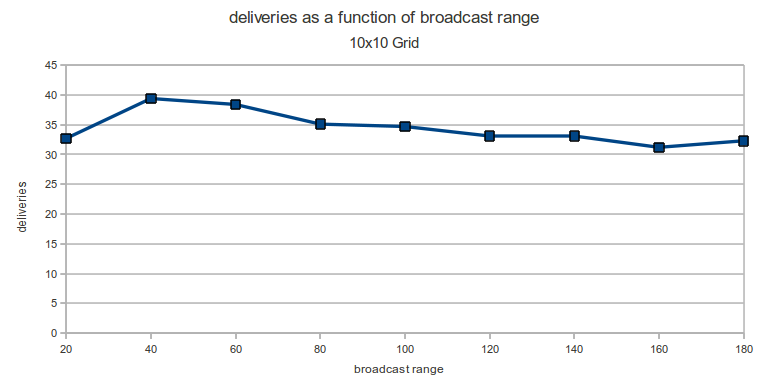
\includegraphics[width=0.8\textwidth]{./figs/grid_broadcastRangeExperiment.png}
		\label{fig:grid_broadcast}
		\caption{Average number of deliveries in function of broadcast range in a
		$10\times10$ grid}
	\end{center}
\end{figure}

\npar A similar setup is used for Leuven. The ``diameter'' of Leuven is a lot
larger than that of the $10\times10$ grid, though. Therefore, increments of 1000
distance units are used. The results are shown in figure
\ref{fig:leuven_broadcast}. Here, the best value seems to be 8000 but as
before, this is not a very significant result.

\begin{figure}[H]
	\begin{center}
		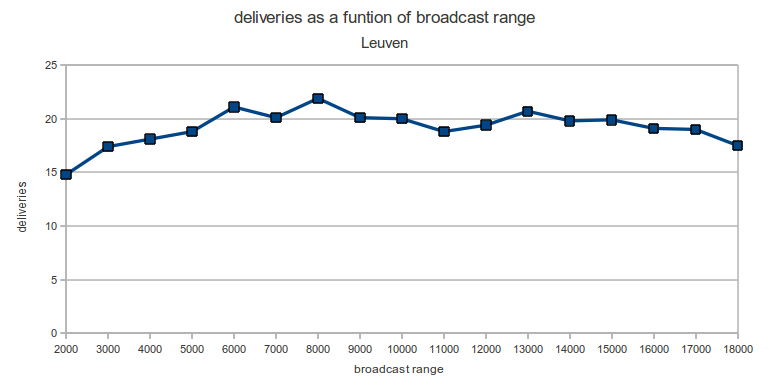
\includegraphics[width=0.8\textwidth]{./figs/leuven_broadcastRangeExperiment.png}
		\label{fig:leuven_broadcast}
		\caption{Average number of deliveries in function of broadcast range in
		Leuven}
	\end{center}
\end{figure}

\npar Now that the ``best'' parameters are determined, the actual comparison can
take place. As before, the same scenario is run 10 times for each strategy
(Gradient Field, Contract Net and Delegate MAS). From these 10 runs, the average
result is calculated. 

\npar For the grid, we see that the Gradient Field offers the best solution,
followed by the Contract Net strategy and the Delegate MAS solution is the least
performing (see figure \ref{fig:deliveries}). However, in a real world
environment like Leuven, the Gradient Field solution performs the worst. The
reason for this is that the trucks easily enter a deadlock state. This can
however still be tweaked by adapting the field strength weights. It is also
possible to remember the last visited nodes and determine whether a truck is
going back and forth in a (dead end) street.

\npar It is remarkable that the Delegate MAS cannot outperform the Contract Net
implementation as we would expect it to do so.

\begin{figure}[H]
	\begin{center}
		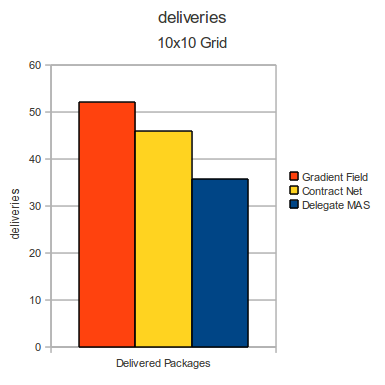
\includegraphics[width=0.4\textwidth]{./figs/grid_deliveries.png}
		\quad
		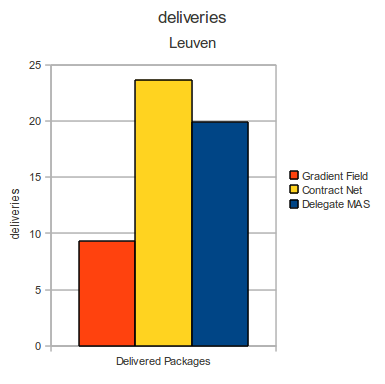
\includegraphics[width=0.4\textwidth]{./figs/leuven_deliveries.png}
		\label{fig:deliveries}
		\caption{Average number of deliveries for every tested strategy}
	\end{center}
\end{figure}

\npar When comparing average distance for a delivery job (see figure
\ref{fig:distances}), there are some obvious remarks. In the grid, a
deadlock will never occur, the travelled distance is thus optimal. In a real
world environment though, deadlocks do occur and the truck travels lots of
miles\ldots

\npar When comparing Contract Net to Delegate MAS, the average distances are
similar. With a little more parameter tweaking, the Delegate MAS solution can
possibly outperform the Contract Net solution. However, this solution can also
be tweaked.

\begin{figure}[H]
	\begin{center}
		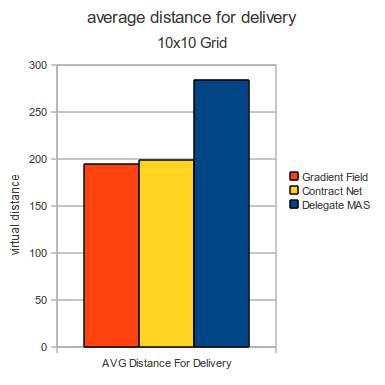
\includegraphics[width=0.4\textwidth]{./figs/grid_distance.png}
		\quad
		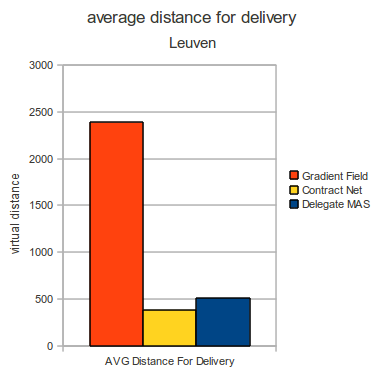
\includegraphics[width=0.4\textwidth]{./figs/leuven_distance.png}
		\label{fig:distances}
		\caption{Average distance for a delivery job for every tested strategy}
	\end{center}
\end{figure}

\npar Finally, the average latenesses and completion times are compared. The
results for the grid are show in figure \ref{fig:grid_times}, the results for
Leuven are shown in figure \ref{fig:leuven_times}. These graphs only show
statistics for the packages that are actually delivered. For instance, it would
be impossible for the Gradient Field to have the lowest delivery lateness while
being deadlocked. Other packages would be waiting too.

\begin{figure}[H]
	\begin{center}
		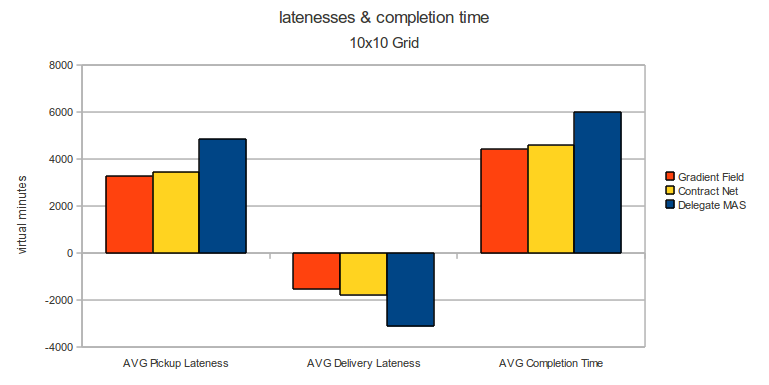
\includegraphics[width=0.8\textwidth]{./figs/grid_times.png}
		\label{fig:grid_times}
		\caption{Average latenesses and completion time for every tested scenario for
		the grid}
	\end{center}
\end{figure}

\begin{figure}[H]
	\begin{center}
		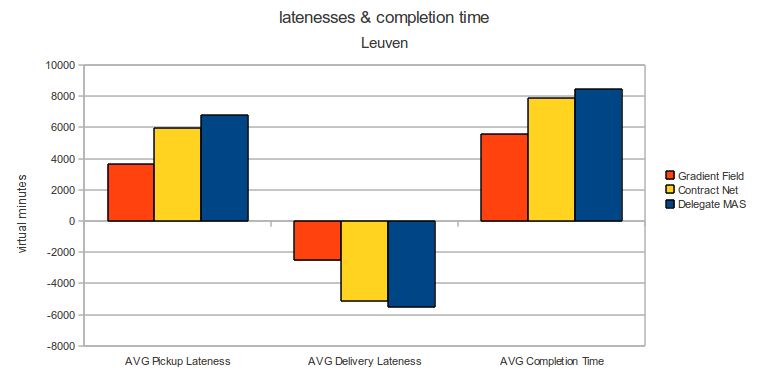
\includegraphics[width=0.8\textwidth]{./figs/leuven_times.png}
		\label{fig:leuven_times}
		\caption{Average latenesses and completion time for every tested scenario for
		Leuven}
	\end{center}
\end{figure}

\npar As you can see, all packages are delivered too late. This is due to the
fact that there are too few trucks to handle this many packages in the used time
window. We could increase the deadline, but it won't change the ranking of the
strategies. You can see that if the trucks manage to deliver packages in a
gradient field, they are delivered the fastest. Next in line is the contract Net
implementation and last is the Delegate MAS solution.

\subsection{Critical Reflection}

\npar First of all, the system manages to get the task done. However, it still
needs a lot of tweaking. 

\npar A huge advantage to this system should be that it can planq ahead, whereas
the (naive) Contract Net and the Gradient Field solution in particular do
not/cannot plan ahead. Using heuristics, the delegate MAS solution can find an
optimal path throughout the system.

\npar One of the disadvantages about this system is that it will not always find
packages at a given moment. Sometimes, it is required to navigate randomly until
packages nearbycan ``hear'' the truck agent. One way to solve this problem would
be to periodically increase the broadcast radius of truck agents (up to a
maximal range) when no packages are found in a certain time window.

\npar Another way to solve this problem could be to combine multiple solutions
into one hybrid solution. When no packages are found, a Gradient Field could be
used to spread the agents accross the physical environment. This will increase
the coverage of the map and hence the chance for packages to be heard by trucks.

\npar As we have seen, traditional systems outperform our delegate MAS solution.
This can probably be optimized by using a better heuristic. To obtain such a
heuristic, more work need to be done, obviously. 

\npar There is however potential and it will scale better than a Contract Net
solution. At this moment, this implementation is pretty naive and broadcasting
means that all agents will receive the message. 

\npar Also, in terms of robustness, we think that Delegate MAS solutions perform
better because they evaporate their pheromones slowly. A missed message will not
result in a missed opportunity.
